\documentclass[letterpaper]{article}
\usepackage[margin=1in]{geometry}

% Set the typeface to Times Roman
\usepackage{times}

%\usepackage{hyperref}
\usepackage{amsfonts}%
\usepackage{amssymb}%
\usepackage{amsthm}% allows theoremstyles (see below) and provides a proof environment
\usepackage{bm}
\usepackage{relsize}
\usepackage{graphicx}
\usepackage{caption}
\usepackage{epstopdf}
\usepackage{amsmath}
\usepackage{tikz}
\usetikzlibrary{trees,arrows}
\usepackage{cite}
\usetikzlibrary{decorations}
\usetikzlibrary[decorations]
\usepgflibrary{decorations.pathmorphing}
\usepgflibrary[decorations.pathmorphing]
\usetikzlibrary{decorations.pathmorphing}
\usetikzlibrary[decorations.pathmorphing]
\usepackage{booktabs}
\usepackage[authoryear]{natbib}
\usepackage{subcaption}
\usepackage{pseudocode}
%\usepackage{float}
\usepackage{verbatim} %% for commenting blocks

\bibpunct{(}{)}{,}{}{}{;} %% added this to make \citep{x} use parentheses

%% independence symbol and expectation operator %%
\newcommand\independent{\protect\mathpalette{\protect\independenT}{\perp}}
\def\independenT#1#2{\mathrel{\rlap{$#1#2$}\mkern2mu{#1#2}}}

\DeclareMathOperator*{\E}{\mathbb{E}}
\DeclareMathOperator*{\Et}{\mathbb{E}_t}
\DeclareMathOperator*{\argmax}{arg\,max}
\DeclareMathOperator{\circlearrow}{\hbox{$\circ$}\kern-1.5pt\hbox{$\rightarrow$}}
\DeclareMathOperator{\circlecircle}{\hbox{$\circ$}\kern-1.2pt\hbox{$--$}\kern-1.5pt\hbox{$\circ$}}

\newcommand\indep{\protect\mathpalette{\protect\independenT}{\perp}}
\def\independenT#1#2{\mathrel{\rlap{$#1#2$}\mkern2mu{#1#2}}}

\newtheorem{Lma}{Lemma}
\newtheorem{Thm}{Theorem}

\DeclareMathOperator*{\Pa}{\text{Pa}}
\DeclareMathOperator*{\Ne}{\text{Ne}}
\DeclareMathOperator*{\Adj}{\text{Adj}}
\DeclareMathOperator*{\Ch}{\text{Ch}}
\DeclareMathOperator*{\An}{\text{An}}
\DeclareMathOperator*{\De}{\text{De}}
\DeclareMathOperator*{\Sp}{\text{Sp}}
\DeclareMathOperator*{\Si}{\text{Si}}
\DeclareMathOperator*{\Nd}{\text{Nd}}
\DeclareMathOperator*{\Mb}{\text{Mb}}
\DeclareMathOperator*{\Cl}{\text{Cl}}
\DeclareMathOperator*{\Bd}{\text{Bd}}

%%%%%%%%%%%%%%%%%%%%%%%%%%%%

\title{Assignment 1}

\author{}

\date{Due: September 20th at 8pm EST}

\begin{document}

\maketitle

	Instructions: This homework requires some calculation, short proofs, and
	programming in R. This is an individual assignment, not group work. Though you may
	discuss the problems with your classmates, you must solve the problems and
	write the solutions independently. As stated in the syllabus, copying code
	from a classmate or the internet (even with minor changes) constitutes
	plagiarism. You are required to submit your answers in pdf form (use \LaTeX)
	in a file called \texttt{<your-UNI>-hw1.pdf} to courseworks. 
	The code for the programming assignment should be appended at the end of this pdf.
	Late submissions will be penalized, except in extenuating circumstances such
	as medical or family emergency. Submissions submitted 0-24 hours late will be
	penalized 10\%, 24-48 hours late by 20\%, 48-72 hours late by 30\%, and later
	than 72 hours by 100\% (i.e., zero credit). The first 4 questions are worth 5 points each, and the
	programming assignment is worth 10 points, for a total of 30 points.

\section*{Problem 1}

Consider the DAG in Figure \ref{fig:prob1}. \\ [3ex]
a) List all the independencies that comprise the local Markov property for this DAG. \\ [3ex]
b) Is $X_2 \perp_d X_9 | X_4$? Is $X_7 \perp_d X_5 | \{X_3, X_8 \}$? Is $ \{X_2, X_4\} \perp_d X_7 | \{X_6, X_9, X_{10} \}$?

\begin{figure}[h]
\begin{center}
\scalebox{0.7}{
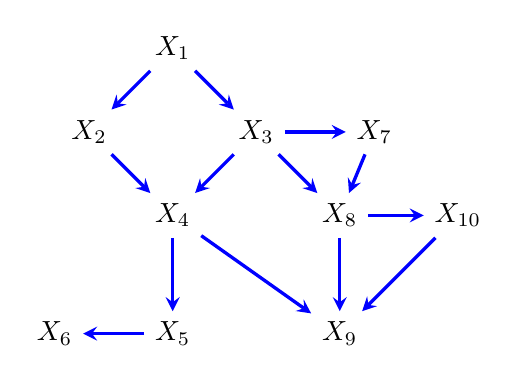
\begin{tikzpicture}[>=stealth, node distance=1.5cm]
    \tikzstyle{format} = [draw, thick, circle, minimum size=1.0mm, inner sep=0pt]
	\tikzstyle{square} = [draw, thick, minimum size=1.0mm, inner sep=3pt]
	\begin{scope}
		\path[->, very thick]
			node[] (x1) {$X_1$}
			node[below left of=x1] (x2) {$X_2$}
			node[below right of=x1] (x3) {$X_3$}		
			node[right of=x3] (x7) {$X_7$}
			node[below right of=x3] (x8) {$X_8$}
			node[below left of=x3] (x4) {$X_4$}
			node[right of=x8] (x10) {$X_{10}$}
			node[below of=x8] (x9) {$X_9$}
			node[below of=x4] (x5) {$X_5$}
			node[left of=x5] (x6) {$X_6$}
			(x1) edge[blue] (x2)
			(x1) edge[blue] (x3)
			(x2) edge[blue] (x4)
			(x3) edge[blue] (x7)
			(x3) edge[blue] (x4)
			(x3) edge[blue] (x8)
			(x4) edge[blue] (x5)
			(x4) edge[blue] (x9)
			(x5) edge[blue] (x6)
			(x7) edge[blue] (x8)
			(x8) edge[blue] (x9)
			(x8) edge[blue] (x10)
			(x10) edge[blue] (x9)
			;
	\end{scope}
\end{tikzpicture}
}
\end{center}
\caption{}
\label{fig:prob1}
\end{figure}


\section*{Problem 2}

In class we defined the Markov blanket of a vertex $X_i$ in DAG $\mathcal{G}$. Show, using d-separation, that this set satisfies $X_i \indep {X} \setminus \{\Mb(X_i,\mathcal{G}), X_i\} | \Mb(X_i, \mathcal{G})$. \\ [2ex]
\small
Hint: you just need to show that the corresponding d-separation holds. Then the independence follows from global Markov property. In general, if someone asks you to prove a certain d-separation holds, one strategy for doing this is proof by contradiction: assume, for the sake of contradiction, that there exists a d-connecting path given the conditioning set and show by definitions (of d-connection and DAG) that this leads to a violation of the assumptions.
\normalsize
\section*{Problem 3}
Consider the two DAGs below. What conditional independence statements do they agree on? Which do they disagree on?
\begin{figure}[h]
	\begin{center}
		\scalebox{0.7}{
			\begin{tikzpicture}[>=stealth, node distance=1.5cm]
				\tikzstyle{format} = [draw, thick, circle, minimum size=1.0mm, inner sep=0pt]
				\tikzstyle{square} = [draw, thick, minimum size=1.0mm, inner sep=3pt]
				\begin{scope}
					\path[->, very thick]
					node[] (A) {$A$}
					node[right of=A] (C) {$C$}
					node[below right of=A, xshift=-0.2cm] (B) {$B$}
					node[below of=B] (D) {$D$}
					(A) edge[blue] (B)
					(C) edge[blue] (B) 
					(B) edge[blue] (D)
					node[below of=D] (l) {$(a)$}	
					;
				\end{scope}
				\begin{scope}[xshift=6.0cm]
					\path[->, very thick]
					node[] (A) {$A$}
					node[below of=A] (B) {$B$}
					node[below right of=B] (D) {$D$}
					node[below left of=B] (C) {$C$}
					(A) edge[blue] (B)
					(B) edge[blue] (C) 
					(B) edge[blue] (D)
					node[below left of=D] (l) {$(b)$}	
					;
				\end{scope}
			\end{tikzpicture}
		}
	\end{center}
\caption{}
\end{figure}

%\clearpage
\section*{Problem 4}
a) Consider the DAG $\mathcal{G}$ in Figure \ref{fig:prob3a}. Which of the DAGs in Figure \ref{fig:prob3b} are Markov equivalent to $\mathcal{G}$? \\ [3ex]
b) How many DAGs are Markov equivalent to the ``chain DAG'' $X_1 \rightarrow X_2 \rightarrow \cdots \rightarrow X_p$ (excluding itself)?

\begin{figure}[h]
\begin{center}
\scalebox{0.7}{
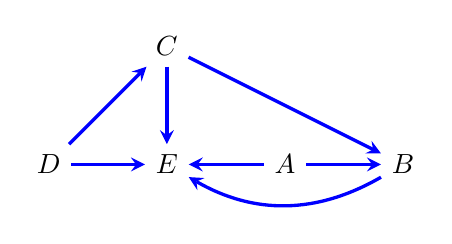
\begin{tikzpicture}[>=stealth, node distance=1.5cm]
    \tikzstyle{format} = [draw, thick, circle, minimum size=1.0mm, inner sep=0pt]
	\tikzstyle{square} = [draw, thick, minimum size=1.0mm, inner sep=3pt]
	\begin{scope}
		\path[->, very thick]
			node[] (C) {$C$}
			node[below of=C] (E) {$E$}
			node[right of=E] (A) {$A$}
			node[left of=E] (D) {$D$}
			node[right of=A] (B) {$B$}
			(A) edge[blue] (B)
			(A) edge[blue] (E) 
			(B) edge[blue, bend left] (E)
			(C) edge[blue] (B)
			(D) edge[blue] (C)
			(D) edge[blue] (E)
			(C) edge[blue] (E)
			;
	\end{scope}
\end{tikzpicture}
}
\end{center}
\caption{}
\label{fig:prob3a}
\end{figure}

\begin{figure}[h]
\begin{center}
\scalebox{0.7}{
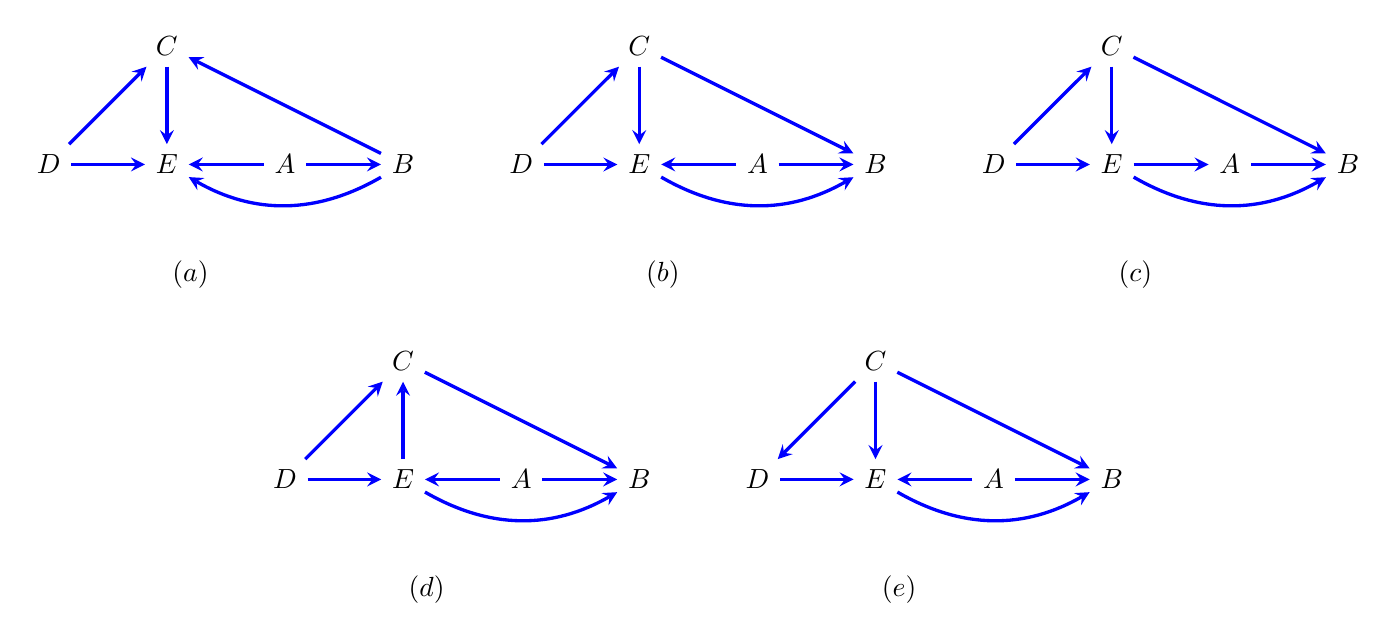
\begin{tikzpicture}[>=stealth, node distance=1.5cm]
    \tikzstyle{format} = [draw, thick, circle, minimum size=1.0mm, inner sep=0pt]
	\tikzstyle{square} = [draw, thick, minimum size=1.0mm, inner sep=3pt]
	\begin{scope}
		\path[->, very thick]
			node[] (C) {$C$}
			node[below of=C] (E) {$E$}
			node[right of=E] (A) {$A$}
			node[left of=E] (D) {$D$}
			node[right of=A] (B) {$B$}
			(A) edge[blue] (B)
			(A) edge[blue] (E) 
			(B) edge[blue, bend left] (E)
			(B) edge[blue] (C)
			(D) edge[blue] (C)
			(D) edge[blue] (E)
			(C) edge[blue] (E)
			node[below of=E, yshift=0.1cm, xshift=0.3cm] (l) {$(a)$}	
			;
	\end{scope}
	\begin{scope}[xshift=6.0cm]
		\path[->, very thick]
			node[] (C) {$C$}
			node[below of=C] (E) {$E$}
			node[right of=E] (A) {$A$}
			node[left of=E] (D) {$D$}
			node[right of=A] (B) {$B$}
			(A) edge[blue] (B)
			(A) edge[blue] (E) 
			(E) edge[blue, bend right] (B)
			(C) edge[blue] (B)
			(D) edge[blue] (C)
			(D) edge[blue] (E)
			(C) edge[blue] (E)
			node[below of=E, yshift=0.1cm, xshift=0.3cm] (l) {$(b)$}	
			;
	\end{scope}
	\begin{scope}[xshift=12.0cm]
		\path[->, very thick]
			node[] (C) {$C$}
			node[below of=C] (E) {$E$}
			node[right of=E] (A) {$A$}
			node[left of=E] (D) {$D$}
			node[right of=A] (B) {$B$}
			(A) edge[blue] (B)
			(E) edge[blue] (A) 
			(E) edge[blue, bend right] (B)
			(C) edge[blue] (B)
			(D) edge[blue] (C)
			(D) edge[blue] (E)
			(C) edge[blue] (E)
			node[below of=E, yshift=0.1cm, xshift=0.3cm] (l) {$(c)$}	
			;
	\end{scope}
	\begin{scope}[xshift=3.0cm, yshift=-4cm]
		\path[->, very thick]
			node[] (C) {$C$}
			node[below of=C] (E) {$E$}
			node[right of=E] (A) {$A$}
			node[left of=E] (D) {$D$}
			node[right of=A] (B) {$B$}
			(A) edge[blue] (B)
			(A) edge[blue] (E) 
			(E) edge[blue, bend right] (B)
			(C) edge[blue] (B)
			(D) edge[blue] (C)
			(D) edge[blue] (E)
			(E) edge[blue] (C)
			node[below of=E, yshift=0.1cm, xshift=0.3cm] (l) {$(d)$}	
			;
	\end{scope}
	\begin{scope}[xshift=9.0cm, yshift=-4cm]
		\path[->, very thick]
			node[] (C) {$C$}
			node[below of=C] (E) {$E$}
			node[right of=E] (A) {$A$}
			node[left of=E] (D) {$D$}
			node[right of=A] (B) {$B$}
			(A) edge[blue] (B)
			(A) edge[blue] (E) 
			(E) edge[blue, bend right] (B)
			(C) edge[blue] (B)
			(C) edge[blue] (D)
			(D) edge[blue] (E)
			(C) edge[blue] (E)
			node[below of=E, yshift=0.1cm, xshift=0.3cm] (l) {$(e)$}	
			;
	\end{scope}
\end{tikzpicture}
}
\end{center}
\caption{}
\label{fig:prob3b}
\end{figure}


\section*{Problem 5}

In this problem you'll get acquainted with using the R package ``dagitty". Being by installing the package and load it into your R session. (You can find basic instructions and tutorials for daggity online: \texttt{http://dagitty.net/primer/}) \\

Construct the DAG in Figure \ref{fig:prob7} as a daggity object. For all tasks below, copy and paste the output of your code into your pdf.\\

a) Using the \texttt{paths()} function, list all paths from $C$ to $H$. \\

b) Use the \texttt{dseparated()} function to determine whether $E \perp_d G | A, B$.\\

c) Using the \texttt{impliedConditionalIndependencies()} function, list the conditional independencies relationships implied by the model. Try this also with the option ``type = all.pairs''. (This might take a while to run.) What explains the difference between these two lists, why is the first one shorter than the second? Consult the documentation of the package.\\

d) Simulate data from this DAG using the \texttt{simulateSEM()} function, which associates the DAG with a linear structural equation model. Set the path coefficient range to $(-0.7, 0.7)$ and the sample size to 10000. Verify with linear regression that the Markov blanket property holds for vertex $B$, i.e., that $\Mb(B,\mathcal{G})$ (use the \texttt{markovBlanket()} function) renders the rest of the variables independent of $B$. You can do this by examining the p-values (or confidence intervals) for all covariates outside the Markov blanket in the regression of $B \sim \Mb(B,\mathcal{G}) + \mbox{remaining covariates}$.

\begin{figure}[h]
	\begin{center}
		\scalebox{0.7}{
			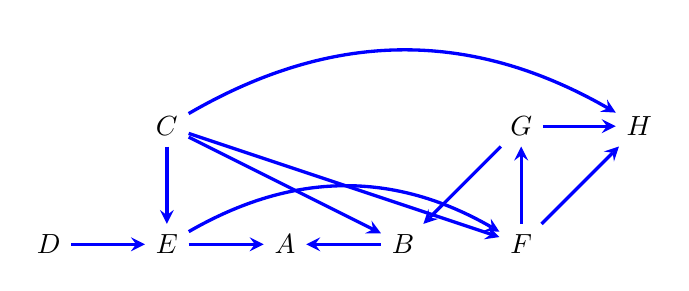
\begin{tikzpicture}[>=stealth, node distance=1.5cm]
			\tikzstyle{format} = [draw, thick, circle, minimum size=1.0mm, inner sep=0pt]
			\tikzstyle{square} = [draw, thick, minimum size=1.0mm, inner sep=3pt]
			\begin{scope}
			\path[->, very thick]
			node[] (C) {$C$}
			node[below of=C] (E) {$E$}
			node[right of=E] (A) {$A$}
			node[left of=E] (D) {$D$}
			node[right of=A] (B) {$B$}
			node[right of = B] (F) {$F$}
			node[above of = F] (G) {$G$}
			node[right of = G] (H) {$H$}
			(B) edge[blue] (A)
			(E) edge[blue] (A) 
			(C) edge[blue] (B)
			(F) edge[blue] (H)
			(D) edge[blue] (E)
			(C) edge[blue] (E)
			(C) edge[blue] (F)
			(C) edge[blue, bend left] (H)
			(G) edge[blue] (H)
			(F) edge[blue] (G)
			(G) edge[blue] (B)
			(E) edge[blue, bend left] (F)
			;
			\end{scope}
			\end{tikzpicture}
		}
	\end{center}
	\caption{}
	\label{fig:prob7}
\end{figure}

\section*{Extra Credit}

Prove the following: in any DAG with $X_i$ not adjacent to $X_j$, necessarily $X_i \perp_d X_j | \{ \Pa(X_i, \mathcal{G}) \cup \Pa(X_j, \mathcal{G}) \}$. Use the definition of d-separation. (Do not simply follow what chatGPT says about this, it is not correct!)


\end{document}
